\documentclass[border=10pt]{article}
\usepackage{tikz}
% we want ER + above/below + left/right
\usetikzlibrary{er,positioning}
\begin{document}
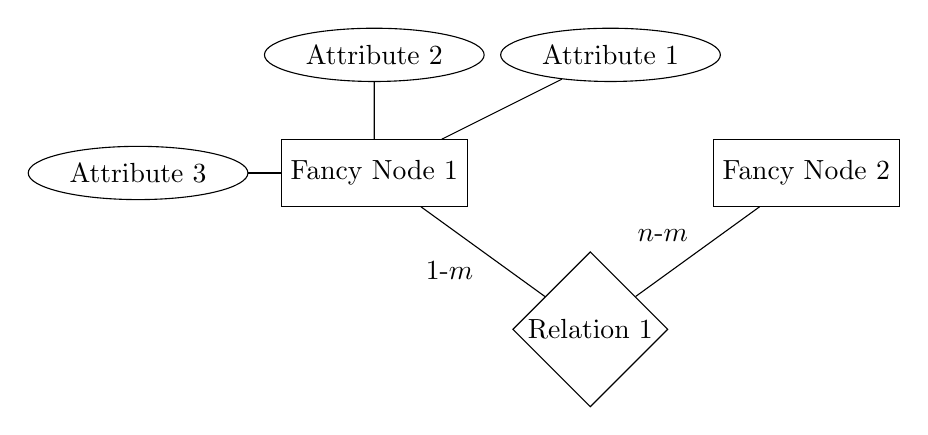
\begin{tikzpicture}[auto,node distance=1.5cm]
  % Create an entity with ID node1, label "Fancy Node 1".
  % Default for children (ie. attributes) is to be a tree "growing up"
  % and having a distance of 3cm.
  %
  % 2 of these attributes do so, the 3rd's positioning is overridden.
  \node[entity] (node1) {Fancy Node 1}
    [grow=up,sibling distance=3cm]
    child {node[attribute] {Attribute 1}}
    child {node[attribute] {Attribute 2}}
    child[grow=left,level distance=3cm] {node[attribute] {Attribute 3}};
  % Now place a relation (ID=rel1)
  \node[relationship] (rel1) [below right = of node1] {Relation 1};
  % Now the 2nd entity (ID=rel2)
  \node[entity] (node2) [above right = of rel1]	{Fancy Node 2};
  % Draw an edge between rel1 and node1; rel1 and node2
  \path (rel1) edge node {1-\(m\)} (node1)
    edge	 node {\(n\)-\(m\)}	(node2);
\end{tikzpicture}
\end{document}